\documentclass[10pt,letterpaper]{article}
\usepackage[utf8]{inputenc}
\usepackage{natbib}
\usepackage{amsmath}
\usepackage{amsfonts}
\usepackage{amssymb}
\usepackage{graphicx}
\usepackage[backgroundcolor=green!20]{todonotes}  % add [disable] before the first bracket to disable all todo commands
% this command enumerates todo notes for better documenting of todo's
\newcounter{todocounter}
\newcommand{\todonum}[2][]
{\stepcounter{todocounter}\todo[#1]{\thetodocounter: #2}}

\author{Baker Potts}

\begin{document}

\section*{Several Ways to Solve the Spring-Mass-Damper Equation of Motion}

\section{Background}
The oft-used equation of motion for a spring mass damper in an inertial frame of reference is
\begin{equation}
	m\ddot{x} + b\dot{x} + kx = F(t)
	\label{eq:smd_eom}
\end{equation}
where $m$ is the mass, $b$ is the damping coefficient, and $k$ is the spring constant.

Solving this differential equation for the spatial positioning of the mass over time given a user-defined forcing ($F(t)$) can be accomplished one of several different methods.

\subsection{Ogata's Derivation}

\subsection{Marion's Derivation}
The equation of motion used by \citet{marion95.1} to describe the spring-mass-damper system is 
\begin{equation}
	\ddot{x} + 2\beta\dot{x} + \omega_0^2 x = \frac{F_0}{m}\cos(\omega t)
\end{equation}
The complementary and particular solution for the position of the mass as a function of time as derived in Section 3.6 by \citet{marion95.1} is
\begin{align}
	x(t) &= x_c(t) + x_p(t) \\
	&= e^{-\beta t} \left[ A_1 e^{\sqrt{\beta^2 - \omega_0^2}t} + A_2 e^{-\sqrt{\beta^2 - \omega_0^2}t} \right] + \frac{F_0/m}{\sqrt{(\omega_0^2-\omega^2)^2 + 4\omega^2\beta^2}}\cos(\omega t - \delta)
\end{align}
where $A_1$ and $A_2$ are determined from initial conditions.
The natural frequency, in the absence of damping, is $\omega_0 = \sqrt{k/m}$.
The damping parameter, $\beta$, is equal to $b/2m$, where $b$ is the damping constant, and the phase difference between the driving force and response is $\delta$.

\subsection{Thomson and Dahleh's Derivation}
From \citet{thomson98.1}:
Differential equation describing the motion:
\begin{equation}
	\ddot{x} + 2\zeta\omega_n \dot{x} + \omega_n^2 x = \frac{F_0}{m}\sin(\omega t)
\end{equation}
Complete solution:
\begin{equation}
	x(t) = \frac{F_0}{k}\frac{\sin(\omega t - \phi)}{\sqrt{\left[1-\left(\frac{\omega}{\omega_n}\right)^2 \right]^2 + \left[2\zeta\frac{\omega}{\omega_n} \right]^2}} + X_1 e^{-\zeta\omega_n t}\sin(\sqrt{1-\zeta^2}\omega_n t + \phi_1)
\end{equation}
where 
\begin{align}
	\omega_n &= \sqrt{\frac{k}{m}} \equiv \text{natural frequency of undamped oscillation} \\
	c_c &= 2m\omega_n \equiv \text{critical damping} \\
	\zeta &= \frac{c}{c_c} \equiv \text{damping factor}
\end{align}

\subsection{Birk's Derivation}

\subsection{Note on Derivations}
Dr. Birk calls his equation 5 or 10 (in name4162f08-05-forcedmotion.pdf) a transfer function, but I disagree with this semantically.
By definition, the transfer function is the ratio of the Laplace transform of the output over the Laplace transform of the input with initial conditions set to 0.
This is defined in Chapter 3 of \citet{ogata01.1}.

%Luke has used the formula from Birk's derivation as the transfer function for his convolution integral method; however, I disagree with this since, by definition, the transfer function is the ratio of the Laplace transform of the output over the Laplace transform of the input with initial conditions set to 0.
%This is defined in Chapter 3 of \citet{ogata01.1}.

Dr. Birk's formulation (eqation 5 or 10) is based on an assumed solution of harmonic response given a harmonic exciting force.

\section{Frequency Domain vs Convolution}
The question continues to arise whether to use the frequency domain method or convolution integral 
Both require a differential equation describing the system, one determined via a Laplace transform with zero initial conditions and unit impulse input.
The other can be called a frequency response function.

Convolution is used if time history is important.
The Laplace-derived transfer function can handle the transients but no arbitrary initial conditions; however, it can handle an arbitrary forcing.
Remember, however, a differential equation can be solved for both the transient and steady-state solutions using a Laplace transform and arbitrary initial conditions and forcing.
This is accomplished by inverse-Laplace transforming into the time domain.

Frequency response function leaves out the phase, and thus the transients, since this function is used mainly when the energy of the system is desired.

\citet{thomson98.1} gives an explanation of the frequency response function which is what Birk ends up deriving, but he does account for the phase which isn't included here.
It's not a transfer function in the strictest sense of the definition since the function is derived from steady-state input.

From pp. 398-400 of \citet{thomson98.1}: ``In the time domain, the system behavior can be determined in terms of the system impulse response $h(t)$ used in the convolution integral.
A much simpler relationship is available for the frequency domain in terms of the frequency response function $H(\omega)$, which we can define as the ratio of the output to the input under \textbf{steady-state} with the input equal to a harmonic time function of unit amplitude.
\textbf{The transient solution is thus excluded in this consideration.}
In random vibrations, the initial conditions and the phase have little meaning and are therefore ignored.
We are mainly concerned with the average energy, which we can associate with the mean square value.
The input-output relationship in terms of the frequency-response function can be written as $y(t) = H(\omega)F_0 e^{i\omega t}$.''

This quoting from Bracewell explains a lot with regards to using the convolution integral versus the frequency domain method.
Paraphrasing, he basically says that although the two methods end up with the same results, the frequency domain method can't `see' into the future.

From pp. 390-3 of \citet{bracewell00.1}: ``In problems where $V_2(t)$ [output response] must be found given $V_1(t)$ [input forcing], two distinct courses must always be borne in mind: one is to proceed by multiplication with the transfer function in the transform domain; the other method is to proceed, by use of the impulse response, directly through the superposition integral.
A strange difference between the two procedures may be noted.
The superposition [convolution] integral does not make use of values of $V_1(t)$ for $t > t_1$ during the course of calculating $V_2(t)$.
In other words, to calculate what is happening now, we need only know the history of excitation up to the present moment.

``But the procedure in the transform domain normally makes use of information about the future excitation.
Indeed, to calculate the Laplace transform of the excitation $V_1(t)$ we have to know its behavior indefinitely into the future.

``As a rule, one obtains the same result for the response at $t=t_1$ irrespective of what $V_1(t)$ does after $t_1$ passes, but occasional trouble can be expected. 
For example, it is perfectly reasonable to ask what is the response of a system to $V_1(t) = e^{t^2}[H(t)]$, and the superposition integral gives it readily, but the Laplace integral diverges because of troubles connected with the infinitely remote future.
One way out of this dilemma is to assume that the excitation is perpetually on the point of ceasing; in other words, assume an excitation $e^{t^2}[H(t) - H(t_1)]$.''

\textbf{Summary:}
\begin{itemize}
	\item frequency response function doesn't account for phases(although Birk's method does)
	\item frequency-response function derived from steady-state input	
	\item Laplace transform and inverse-Laplace can be used to compute the transient solution of a differential equation given initial conditions and arbitrary forcing
	\item diff. eg. in time $\Rightarrow$ Laplace transform $\Rightarrow$ specify initial conditions and forcing $\Rightarrow$ inverse-Laplace to get full, unique solution
	\item Laplace-derived transfer function with ZIC (zero initial conditions) gives a frequency domain solution that can be used to obtain the transient solution given an arbitrary forcing; however, arbitrary initial conditions cannot be applied
	\item convolution integral is the surest method of computing the system output time-domain response given initial conditions
\end{itemize}

\section{Laplace Transform Method}
With zero initial conditions, this equation can be transformed into the Laplace (frequency) domain using Laplace transformation:
\begin{equation}
	ms^2 X(s) + bsX(s) + kX(s) = F(s)
\end{equation}
and rearranged into transfer function form which is the output over input
\begin{equation}
	\frac{X(s)}{F(s)} = \frac{1}{ms^2 + bs + k}
\end{equation}
Multiplying an input forcing of $F(s)$ with the right hand side of this last equation gives the output $X(s)$.
This output can then be inverse-Laplace transformed into the time domain to get the time-series response of the spring-mass-damper to a forcing of $F(t)$.

Consider an input forcing of a unit impulse function at $t=t_a$:
\begin{equation}
	F_{imp}(t) = \delta(t-t_a)
\end{equation}
Transforming into the Laplace domain gives
\begin{equation}
	F_{imp}(s) = e^{-t_a s}
\end{equation}

Multiplying $F_{imp}$ by the transfer function from above gives the output
\begin{equation}
	Y(s) = \frac{e^{-t_a s}}{ms^2 + bs + k}
\end{equation}
in the frequency domain.
Taking the inverse-Laplace transform gives the solution in the time domain.
This is accomplished with partial fraction decomposition and the 2nd shift formula:
\begin{equation}
	y(t) =
	\begin{cases}
		0 & \text{if } 0 \leq t < t_a \\
		-\frac{1}{d}e^{-(\frac{b+d}{2m})(t-t_a)} + \frac{1}{d}e^{-(\frac{b-d}{2m})(t-t_a)} & \text{if } t\geq t_a
	\end{cases}
\end{equation}
where $d=\sqrt{b^2 - 4km}$.

Using the parameters of Case 1 (Table \ref{tab:parameters}), the time-domain response to the unit impulse at $t_a=2\text{ s}$ is plotted in Figure \ref{fig:laplacesolution}.
\begin{figure}
	\centering
	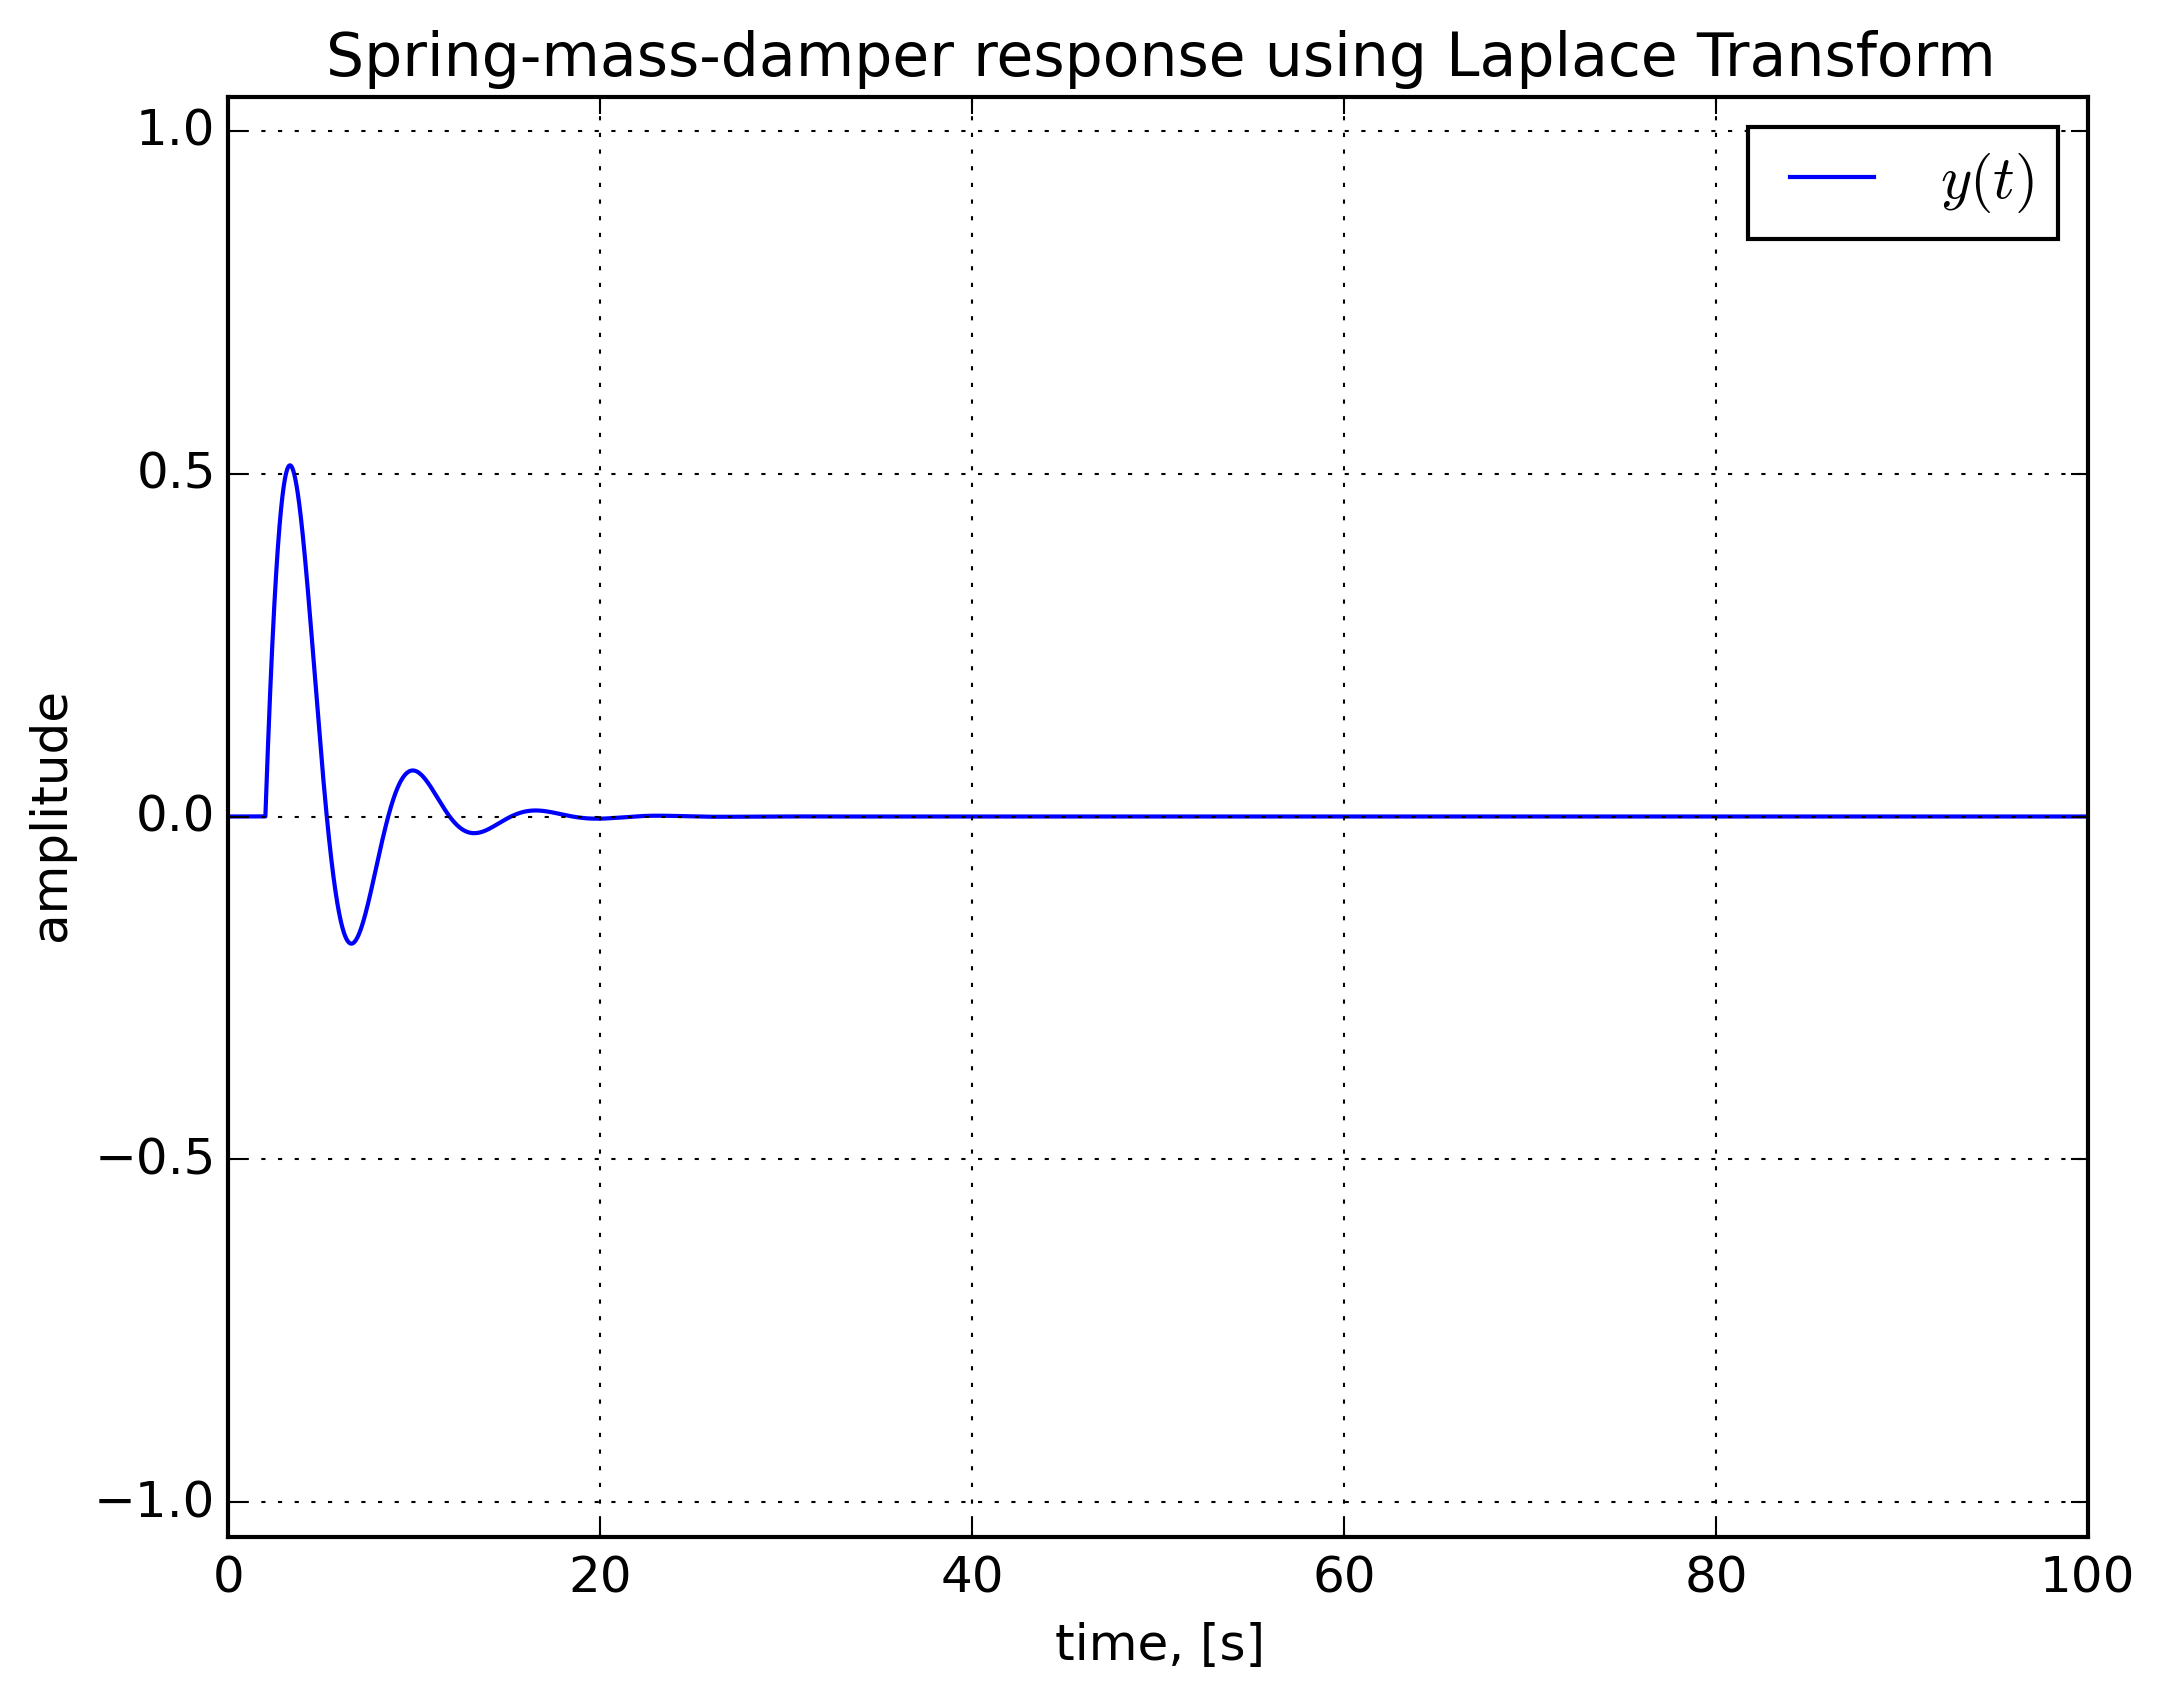
\includegraphics[width=\textwidth, height=\textheight, keepaspectratio]{./laplacesolution.png}
	\caption{Response to an impulse at $t_a=2\text{ s}$.}
	\label{fig:laplacesolution}
\end{figure}

\section{Root-Locus Analysis}
The basic characteristic of the transient response of a closed-loop system is closely related to the location of the closed-loop poles.
Root locus analysis is a mathematical tool that allows one to investigate the pole locations of the closed-loop system as parametrized by the gain of the feedback system.

This system differs from the other examples in that it is a closed-loop one.
The output of the system is controlled to match a user-defined setpoint as opposed to simply inputting a forcing to the system and computing its response.
It is assumed that the measurement of the output is known (in a real situation, the output measurement is obtained via a sensor).
The dimensions of the gain must agree with the error measurement in that it converts the error into the signal input needed for the system plant, e.g. an armature voltage that controls the torque of a PMDC motor.

Nonetheless, this technique can be used to observe the response of a system, with the goal of restricting the system to a stable domain.
The stability, or constrained oscillations, is ensured if the poles and zeros of the characteristic polynomial are located in the left half of the $s$-plane.

The graphics in Figures \ref{fig:smd_rootlocus_characteristics_kuo}, \ref{fig:constant_loci_plots}, and \ref{fig:step-response_comparisons_of_various_root_locations} are obtained from \citet{kuo10.1}.
Figure \ref{fig:smd_rootlocus_characteristics_kuo} shows the root-locus characteristics of a 2nd order oscillatory system with unity feedback.

\begin{figure}
	\centering
	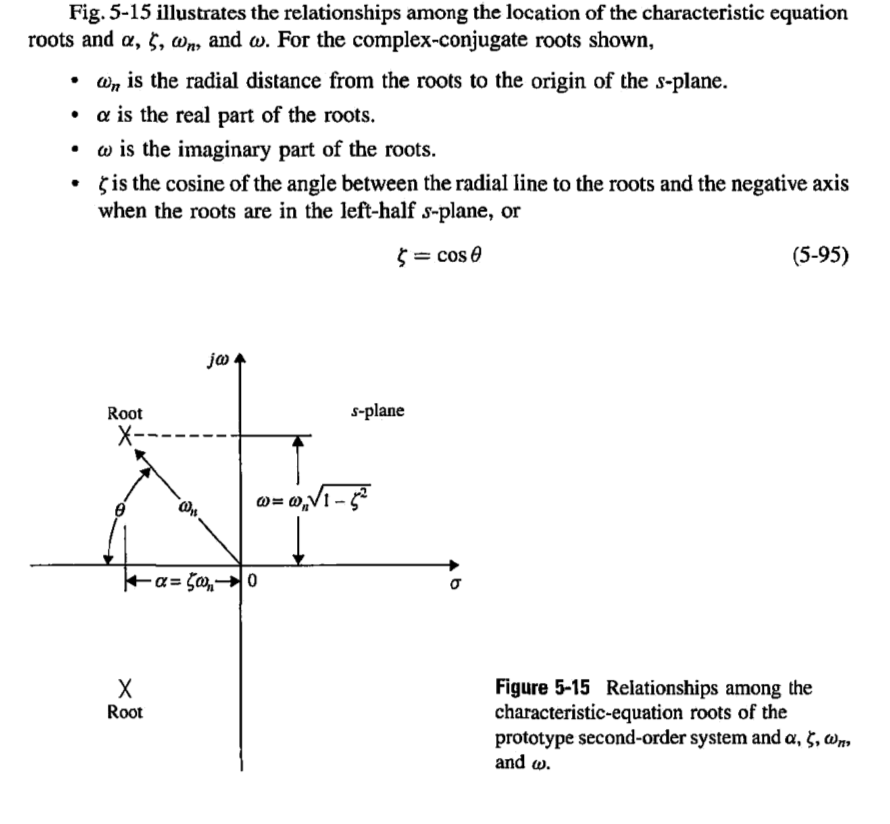
\includegraphics[width=\textwidth, height=\textheight, keepaspectratio]{smd_rootlocus_characteristics_kuo.png}
	\caption{Root-locus characteristics in the $s$-plane (\citet{kuo10.1}).}
	\label{fig:smd_rootlocus_characteristics_kuo}
\end{figure}

Figure \ref{fig:constant_loci_plots} shows the lines on root-locus plots that denote constant damping, etc.

\begin{figure}
	\centering
	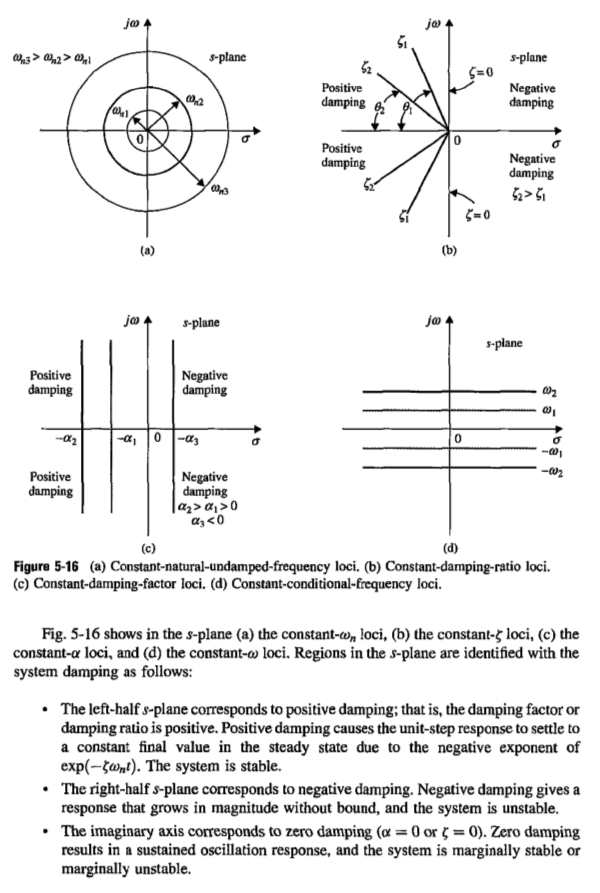
\includegraphics[width=\textwidth, height=\textheight, keepaspectratio]{constant_loci_plots.png}
	\caption{Lines showing various constant loci positions in the $s$-plane (\citet{kuo10.1}).}
	\label{fig:constant_loci_plots}
\end{figure}

Figure \ref{fig:step-response_comparisons_to_various_root_locations} shows the step response comparison of various characteristic equation root locations in the $s$-plane.

\begin{figure}
	\centering
	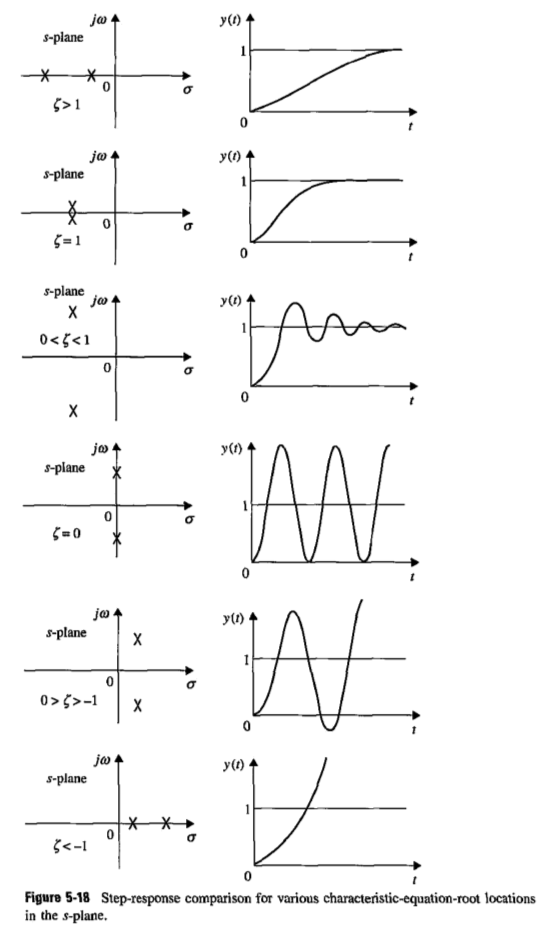
\includegraphics[width=\textwidth, height=0.9\textheight, keepaspectratio]{step-response_comparisons_of_various_root_locations.png}
	\caption{Step response plots of various characteristic equation root locations in the $s$-plane (\citet{kuo10.1}).}
	\label{fig:step-response_comparisons_of_various_root_locations}
\end{figure}

\section{Convolution Method}

\section{Runge-Kutta Integration Method}
Equation \ref{eq:smd_eom} can be rearranged for the highest order state variable, $\ddot{x}$, in order to be placed in a form to be solved using the Runge-Kutta integration method:
\begin{equation}
	\ddot{x} = \frac{1}{m}\left[ F(t) - b\dot{x} - kx \right)]
\end{equation}

The above equation is written as the following system of first-order equations
\begin{align}
	\dot{x_0} &= \frac{1}{m}\left[ F(t) - bx_0 - kx_1 \right)] \\
	\dot{x_1} &= x_0
\end{align}

The variables $\dot{x_0}$ and $\dot{x_1}$ are used in formulas to obtain agreement with a Taylor series solution up to the 4th order terms.
The variable $x_0$ denotes the speed of the mass, and $x_1$ denotes the displacement.
These two state variables are outputted using a recurrence formula based on $\dot{x_0}$ and $\dot{x_1}$ inputs after each integration step of the Runge-Kutta scheme and used as initial conditions for the next integration step.

\section{Green's Method}
This method is paraphrased from Section 3.10 of \citet{marion95.1}:
``Green's method is based on representing an arbitrary forcing function as a series of impulses.
If the driven system is linear, the principle of superposition is valid, and we can express the inhomogeneous part of the differential equation as the sum of individual forcing functions $F_n(t)/m$, which in Green's method are impulse functions.''

For a damped oscillator described by the equation of motion
\begin{equation}
	\ddot{x} + 2\beta\dot{x} + \omega_0^2 x = \frac{F(t)}{m}
\end{equation}
the position in time is defined as
\begin{equation}
	x(t) = \int_{-\infty}^t F(t^{\prime})G(t,t^{\prime})dt^{\prime}
\end{equation}
where $G(t,t^{\prime})$ is known as Green's function for the linear oscillator equation.
Green's function is unique to the system being studied.
For the damped linear oscillator initially at rest at equilibrium, $G(t,t^{\prime})$ is
\begin{equation}
	G(t,t^{\prime}) \equiv 
\begin{cases}
	\frac{1}{m\omega_1}e^{-\beta(t-t^{\prime}}\sin \omega_1(t-t^{\prime}) & t \geq t^{\prime} \\
	0 & t < t^{\prime}
\end{cases}
\end{equation}
and $F(t^{\prime})$ is 
\begin{equation}
	F(t^{\prime}) = ma(t^{\prime})
\end{equation}
The damped frequency of oscillation, $\omega_1$, is
\begin{equation}
	\omega_1 = \sqrt{\beta^2 - \omega_0^2}
\end{equation}

From \citet{marion95.1}: ``Green's method is generally useful for solving linear, inhomogenous differential equations.
The main advantage of the method lies in the fact that the Green's function $G(t,t^{\prime})$, which is the solution of the equation for an infinitesimal element of the inhomogenous part, already contains the initial conditions---so the general solution, expressed by the integral of $F(t^{\prime})G(t,t^{\prime})$, automatically also contains the initial conditions.''

\textbf{Requirements for this method:}
\begin{itemize}
	\item linear (generally)
	\item homogenous or non-homogeneous
	\item initial conditions
\end{itemize}

\section{Parameter Values}
\begin{table}[H]
\centering
\caption{Parameter values for cases used.}
\label{tab:parameters}
\begin{tabular}{ccccc}
       & \multicolumn{4}{c}{Parameters}                        \\ \hline
       & m {[}kg{]} & b {[}N-s/m{]} & k {[}N/m{]} & F(t)       \\ \hline
Case 1 & 1.3        & 0.8           & 1.3         & 2 impulses \\ \hline
Case 2 &            &               &             &           \\ \hline
\end{tabular}
\end{table}

% Bibliography
\bibliographystyle{apalike}
\bibliography{Potts_bibliography}   % Use the BibTeX file ``***.bib''.

\end{document}